\section{Free topic choice without frictions}\label{sec:frictionless}

We first set $b_c=\infty$, so $w=v$. Newcomers move freely between topics and
the frontier. This benchmark isolates the topic-choice margin.

\begin{proposition}[Equilibrium and dissipation]\label{prop:eq}
Let \cref{ass:Q,ass:phi,ass:credit,ass:interior} hold and $b_c=\infty$, and
suppose $\vhat>F(N/n(\Phat),\Phat)$. Then a topic equilibrium exists and is
unique. Every open topic sits on the falling side of the payoff curve,
$P^*>\Phat$, where an additional paper lowers the payoff of every member
(\cref{prop:externality}). Output per researcher equals the frontier value,
$a\,F<a\,\vhat$. The gain from cumulative knowledge, $\vhat-F$, is competed away.
With founders who stay and $\eta_F=0$, the equilibrium density solves
$v(P^*)=e$, whatever the founders' probability $\omega$.
\end{proposition}

Entry continues past the peak because a newcomer compares the \emph{average}
payoff in a topic with the frontier. She ignores that her papers lower everyone
else's payoff once the topic is past $\Phat$. Crossings on the rising side are
unstable: one more entrant raises the payoff of entering. So topics fill past
the peak, to the crossing on the falling side. Founders do not change this.
They earn the same $v(P^*)$ as incumbents, so indifference between founding and
joining pins $v(P^*)$ to what explorers produce.

\begin{remark}[Cities, clubs and topics]\label{rem:henderson}
\Cref{prop:eq,prop:planner} have the structure of the theory of city sizes
\citep{henderson1974} and of clubs \citep{buchanan1965,scotchmer2002}: a single-peaked
average payoff in group size, free entry of new groups, stability only on the
falling side, a planner at the peak of the average payoff, and an entry tax
that decentralises it. Self-organised cities are too large for the same
reason \citep{hendersonbecker2000}. Topics are the cities, newcomers the
migrants, and the frontier the hinterland where new cities are founded. Three
things distinguish topics. The hump is not assumed but derived from the two
jobs of reading (\cref{thm:v}). The congestion is not in land or roads but in
attention: the crowders are the readers, so whether an extra member helps or
hurts is decided by where the topic sits on its payoff curve
(\cref{prop:externality}). And the object the data measure, the duplication rate,
is a function of density alone, which makes the invariance of
\cref{prop:volume} a testable restriction rather than a curiosity.
\end{remark}

\paragraph{Volume opens new topics.} The next result says how a larger
community distributes itself.

\begin{proposition}[Volume opens new topics]\label{prop:volume}
In the large-topic limit, equilibrium density depends on $(N,a)$ only through
the product $N a$, and
\begin{equation}\label{eq:E}
\mathcal E\equiv\frac{\dd\ln P^*}{\dd\ln N}=\frac{\eta_F}{\eta_F\,D+|\eps_w|+\theta_F\,\eps_U},\qquad D\equiv1-\eps_x+\frac{\rho}{\delta}\,\frac{P^*/b_c}{1-P^*/b_c}\ge 1,
\end{equation}
where $\eps_w=\dd\ln w/\dd\ln P<0$, $\eps_x=\dd\ln x^*/\dd\ln P\le 0$ and
$\eps_U=\dd\ln\bar U_F/\dd\ln P$ are evaluated at $P^*$ ($\eps_U=\eps_v$ in the
stationary economy). New topics absorb a share $\dd\ln M^*/\dd\ln N=1-D\,\mathcal E$
of growth, and papers per researcher move with elasticity $\eps_x\mathcal E\le 0$.
If the frontier is not depleted ($\eta_F=0$), density, the overlap rate and the
aware share do not depend on $N$, $a$ or the cost of entering science.
\end{proposition}

\Cref{eq:E} holds for any $b_c$, and we use it again in
\cref{sec:catchup,sec:ai}. Three remarks.

First, the overlap rate is \emph{pinned by entry, not by volume}. When the
community grows, newcomers open new topics until existing ones are no more
attractive than the frontier. The flagged overlap rate and the aware share are
functions of $P^*$ alone (\cref{lem:credit}), so they inherit its invariance. A
flat overlap rate while submissions double (Fact~\ref{fact:volume}) is what the
model predicts. It is not evidence that crowding is harmless.

Second, a fixed field corresponds to $\eta_F\to\infty$. Then $\mathcal E\to1/D$:
growth thickens existing topics. The arXiv elasticities of 0.12--0.19 at broad
radii and 0.035 (SE 0.118) at the closest-overlap radius, against fixed-field
benchmarks of 0.53--0.81 (Fact~\ref{fact:volume}), imply that most growth opens
new ground. Inverting \eqref{eq:E},
\begin{equation}\label{eq:eta}
\eta_F=\frac{\mathcal E\,\big(|\eps_w|+\theta_F\eps_U\big)}{1-\mathcal E\,D},
\end{equation}
so the frontier's depletion is identified by the volume elasticity, the slope
of the newcomer's payoff curve and the founders' share. The inversion assumes
that the frontier did not move for other reasons over the sample. A frontier
that improved, for instance because founding got easier, would lower measured
density growth and bias $\eta_F$ down (\cref{thm:incidence}).

Third, papers per author barely move when the community grows, because
$\eps_x\mathcal E$ is the product of two small numbers. Faster production, by
contrast, raises papers per author one for one (\cref{prop:ai}). The two can
be told apart only at the author level, because entrants change the
composition of authors (Fact~\ref{fact:authors}).

\begin{remark}[Short-run and long-run elasticities]\label{rem:shortrun}
\Cref{prop:volume} compares steady states, while the arXiv elasticities are
measured over 2018--2025, a period in which volume grew about 12\% a year. In
the model, mature topics adjust to a change in $N$ at once, since the marginal
newcomer is indifferent. The only wedge between the measured and the
steady-state elasticity is composition. Faster growth means more young topics,
which are thinner. If an area's growth rate rises by $\dd g$ for $T$ years,
its age weights for topics younger than $T$ scale by $e^{\dd g(T-a)}$ and its
log volume rises by $T\dd g$, so
\begin{equation}\label{eq:shortrun}
\mathcal E_{\text{measured}}=\mathcal E+\frac{\operatorname{Cov}_\omega\big(\ln P,(T-a)^+\big)}{T}+o(\dd g),
\end{equation}
where $\operatorname{Cov}_\omega$ is the researcher-weighted covariance over the
cross-section of topic ages $a$. The covariance is negative because young topics
are thin, so the measured elasticity is a lower bound. In the calibrated
life cycle the bias over a seven-year window is $-\calCompBias$
(\cref{sec:quant}). The long-run elasticity is therefore at most about
$\calCompBias$ above the measured one, which leaves the conclusion that
volume mostly opens new ground intact. Steady growth at a constant rate does
not bias the estimate at all, because area fixed effects absorb a constant age
composition.
\end{remark}

\begin{remark}[Reading capacity per researcher or per field]
Consider instead a fixed screening capacity $B$ per field, so that coverage is
$B/P$ and researchers produce full time. Topic choice still pins density, so
\cref{prop:eq,prop:volume} survive. But if topics cannot split, overlap rises
with field volume, which the arXiv volume test rejects. Per-researcher
capacity also keeps the time-allocation margin that prices tools by the time
they save (\cref{lem:timeshares}). We adopt it throughout.
\end{remark}

\begin{figure}[t]
\centering
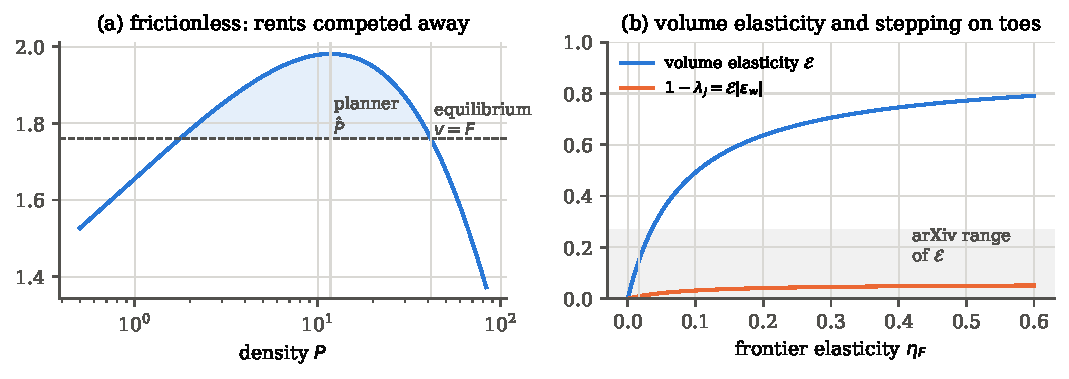
\includegraphics[width=\textwidth]{figures/fig2_planner_volume.pdf}
\caption{Left: without catch-up costs, topics fill to the density where $v=F$,
and the shaded rent between the payoff curve and the frontier is competed away;
the planner puts topics at the peak. Right: the volume elasticity
$\mathcal E$ and the stepping-on-toes wedge $\mathcal E|\eps_w|$ as functions of
the frontier's depletion $\eta_F$, at the calibrated slope of $w$ and founders'
share. The shaded band is the range of arXiv estimates of $\mathcal E$.}
\label{fig:planner}
\end{figure}

\paragraph{The planner.} A planner who controls how many researchers join each
topic, but not how they split their time, maximises output subject to births
equalling deaths and researchers adding up.

\begin{proposition}[Overcrowding and the frontier subsidy]\label{prop:planner}
Let the conditions of \cref{prop:eq} hold, with $b_c\le\infty$ and $\eta_F=0$.
\begin{enumerate}[label=(\roman*)]
\item In the large-topic limit output per researcher at any common density is $a\,w(P)$, so the planner puts every topic at the peak of the newcomer's payoff curve, $P^o=\hat P_w$, which is the peak of $v$ when $b_c=\infty$. She opens more topics and puts fewer researchers in each. The gain in output per researcher is $\hat w/F-1$.
\item With explorers counted and founders who do not stay ($\omega=0$), the planner's density satisfies
\begin{equation}\label{eq:plannerfoc}
\frac{w(P^o)-e}{w(P^o)}=|\eps_w(P^o)|\,\frac{1+s\,n(P^o)/\xi}{D(P^o)},
\end{equation}
with $\hat P_w<P^o<P^*$. Overlap stays positive at the optimum.
\item In the stationary economy a frontier subsidy (equivalently, a tax on joining open topics) of $s^o=\hat w-F(M^o,\hat P_w)$ per unit of production speed decentralises the large-topic optimum.
\item (Two wedges) A planner who also chooses $x$ wants researchers to produce less than $x^*(P)$ wherever $w'(P)<0$ and more wherever $w'(P)>0$. The production wedge is proportional to $(\ln w)'(P)$. In the large-topic limit it vanishes at the optimal density, so controlling topic choice alone attains the first best.
\end{enumerate}
\end{proposition}

There are two wedges, and they differ in importance. Newcomers choose topics
on the average payoff while the planner uses the marginal one: this is the
\emph{crowding wedge}. Inside each topic, researchers ignore that their papers
add to what colleagues must read: this is the \emph{production wedge}. Part
(iv) shows the production wedge is a symptom of the crowding wedge. Once topics
are at their best density, researchers' private time allocation is efficient.
Part (iii) holds in the stationary economy. In an economy where topics are born
thin and grow, a flat subsidy to the frontier also deters the first followers
of newborn topics, and the policy has to depend on a topic's age
(\cref{prop:policy}). The welfare criterion here is total private credit;
\cref{prop:social} shows that the overcrowding result survives when part of
that credit is a transfer, and \cref{prop:audience} values output by
readership instead.
